\section{Est�ndares de codificaci�n}
Entendemos como est�ndar de c�digo a un conjunto de convenciones establecidas de ante mano (denominaciones, formatos, etc.) para la escritura de c�digo \citep{vera2019mejores}.

\paragraph{Comentario de c�digo:}
\begin{itemize}
    \item Los comentarios deben ser oraciones completas.
    \item Si un comentario es una frase u oraci�n su primera palabra debe comenzar con may�scula a menos que sea un identificador que comience con min�scula.
\end{itemize}
\begin{figure}[htp]
    \centering
    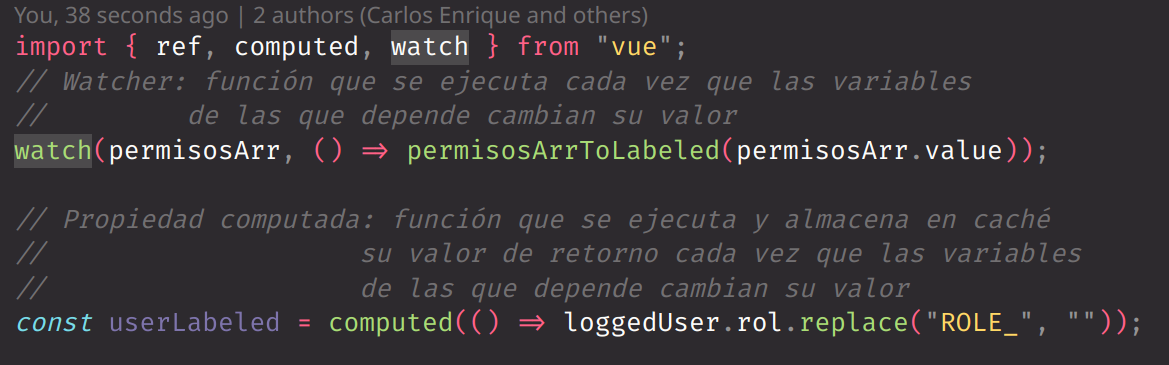
\includegraphics[width=0.6\textwidth]{images/patterns/watch.png}
    \caption{Ejemplo de comentarios en el c�digo fuente de la aplicaci�n cliente}
\end{figure}

\paragraph{M�xima longitud de las l�neas:}

\begin{itemize}
    \item Se limitar�n todas las l�neas a un m�ximo de 150 caracteres.
    \item Dentro de par�ntesis, corchetes o llaves se puede utilizar la continuaci�n impl�cita para cortar las l�neas largas.
\end{itemize}

\paragraph{L�neas en blanco:}
\begin{itemize}
    \item Las definiciones de m�todos dentro de una clase deben separarse por una l�nea en blanco.
    \item Se puede utilizar l�neas en blanco escasamente para separar secciones l�gicas.
\end{itemize}

\paragraph{Importaciones:}
\begin{itemize}
    \item Las importaciones deben estar en l�neas separadas.
    \item Las importaciones siempre deben colocarse al comienzo del archivo.
\end{itemize}
\begin{figure}[htp]
    \centering
    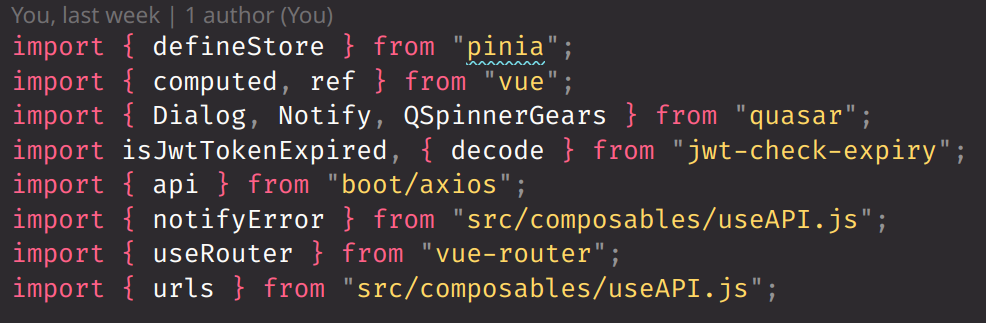
\includegraphics[width=0.6\textwidth]{images/patterns/imports.png}
    \caption{Ejemplo de importaciones al inicio en el c�digo fuente de la aplicaci�n cliente}
\end{figure}